\documentclass[11pt]{article}

\usepackage[english]{babel}
\usepackage[utf8]{inputenc}
\usepackage{geometry}
\usepackage[pdftex]{graphicx}
\usepackage{tabularx}
\usepackage{placeins}

%bib options
\usepackage[backend=biber,style=authoryear,bibstyle=authoryear,natbib=true,
giveninits=true,uniquename=false,uniquelist=false,maxcitenames=2,date=year,
maxbibnames=99,url=false]{biblatex}
\addbibresource{Article.bib}
\usepackage{dsfont}
\usepackage{multirow}
\usepackage{amsmath,amsfonts,amssymb}
\usepackage{subcaption}
\usepackage{authblk}
%hyperlinks options
\usepackage{hyperref}
\hypersetup{colorlinks=true,linkcolor=blue,filecolor=magenta, urlcolor=cyan,citecolor=cyan}
\geometry{a4paper, total={180mm,257mm}, left=20mm, top=20mm}

\title{Supplementary material of the article "Are historical stage records useful to decrease the uncertainty of flood frequency analysis ? A 200-year long case study" from Journal of Hydrology}

\author[1]{Mathieu LUCAS \thanks{Corresponding author at: INRAE, 5 Rue de la Doua, 69100 VILLEURBANNE, FRANCE. \newline E-mail adress: mathieu.lucas@inrae.fr (M. Lucas).}}
\author[2]{Benjamin RENARD}
\author[1]{Jérôme LE COZ}
\author[1]{Michel LANG}
\author[3]{Antoine BARD}
\author[4]{Gilles PIERREFEU}
\affil[1]{INRAE, UR RIVERLY, Villeurbanne, France}
\affil[2]{INRAE, UR RECOVER, Aix-en-Provence, France}
\affil[3]{ESDB, Briançon}
\affil[4]{CNR, Lyon}

\begin{document}

\maketitle


	\begin{figure}[h]
		\centering
		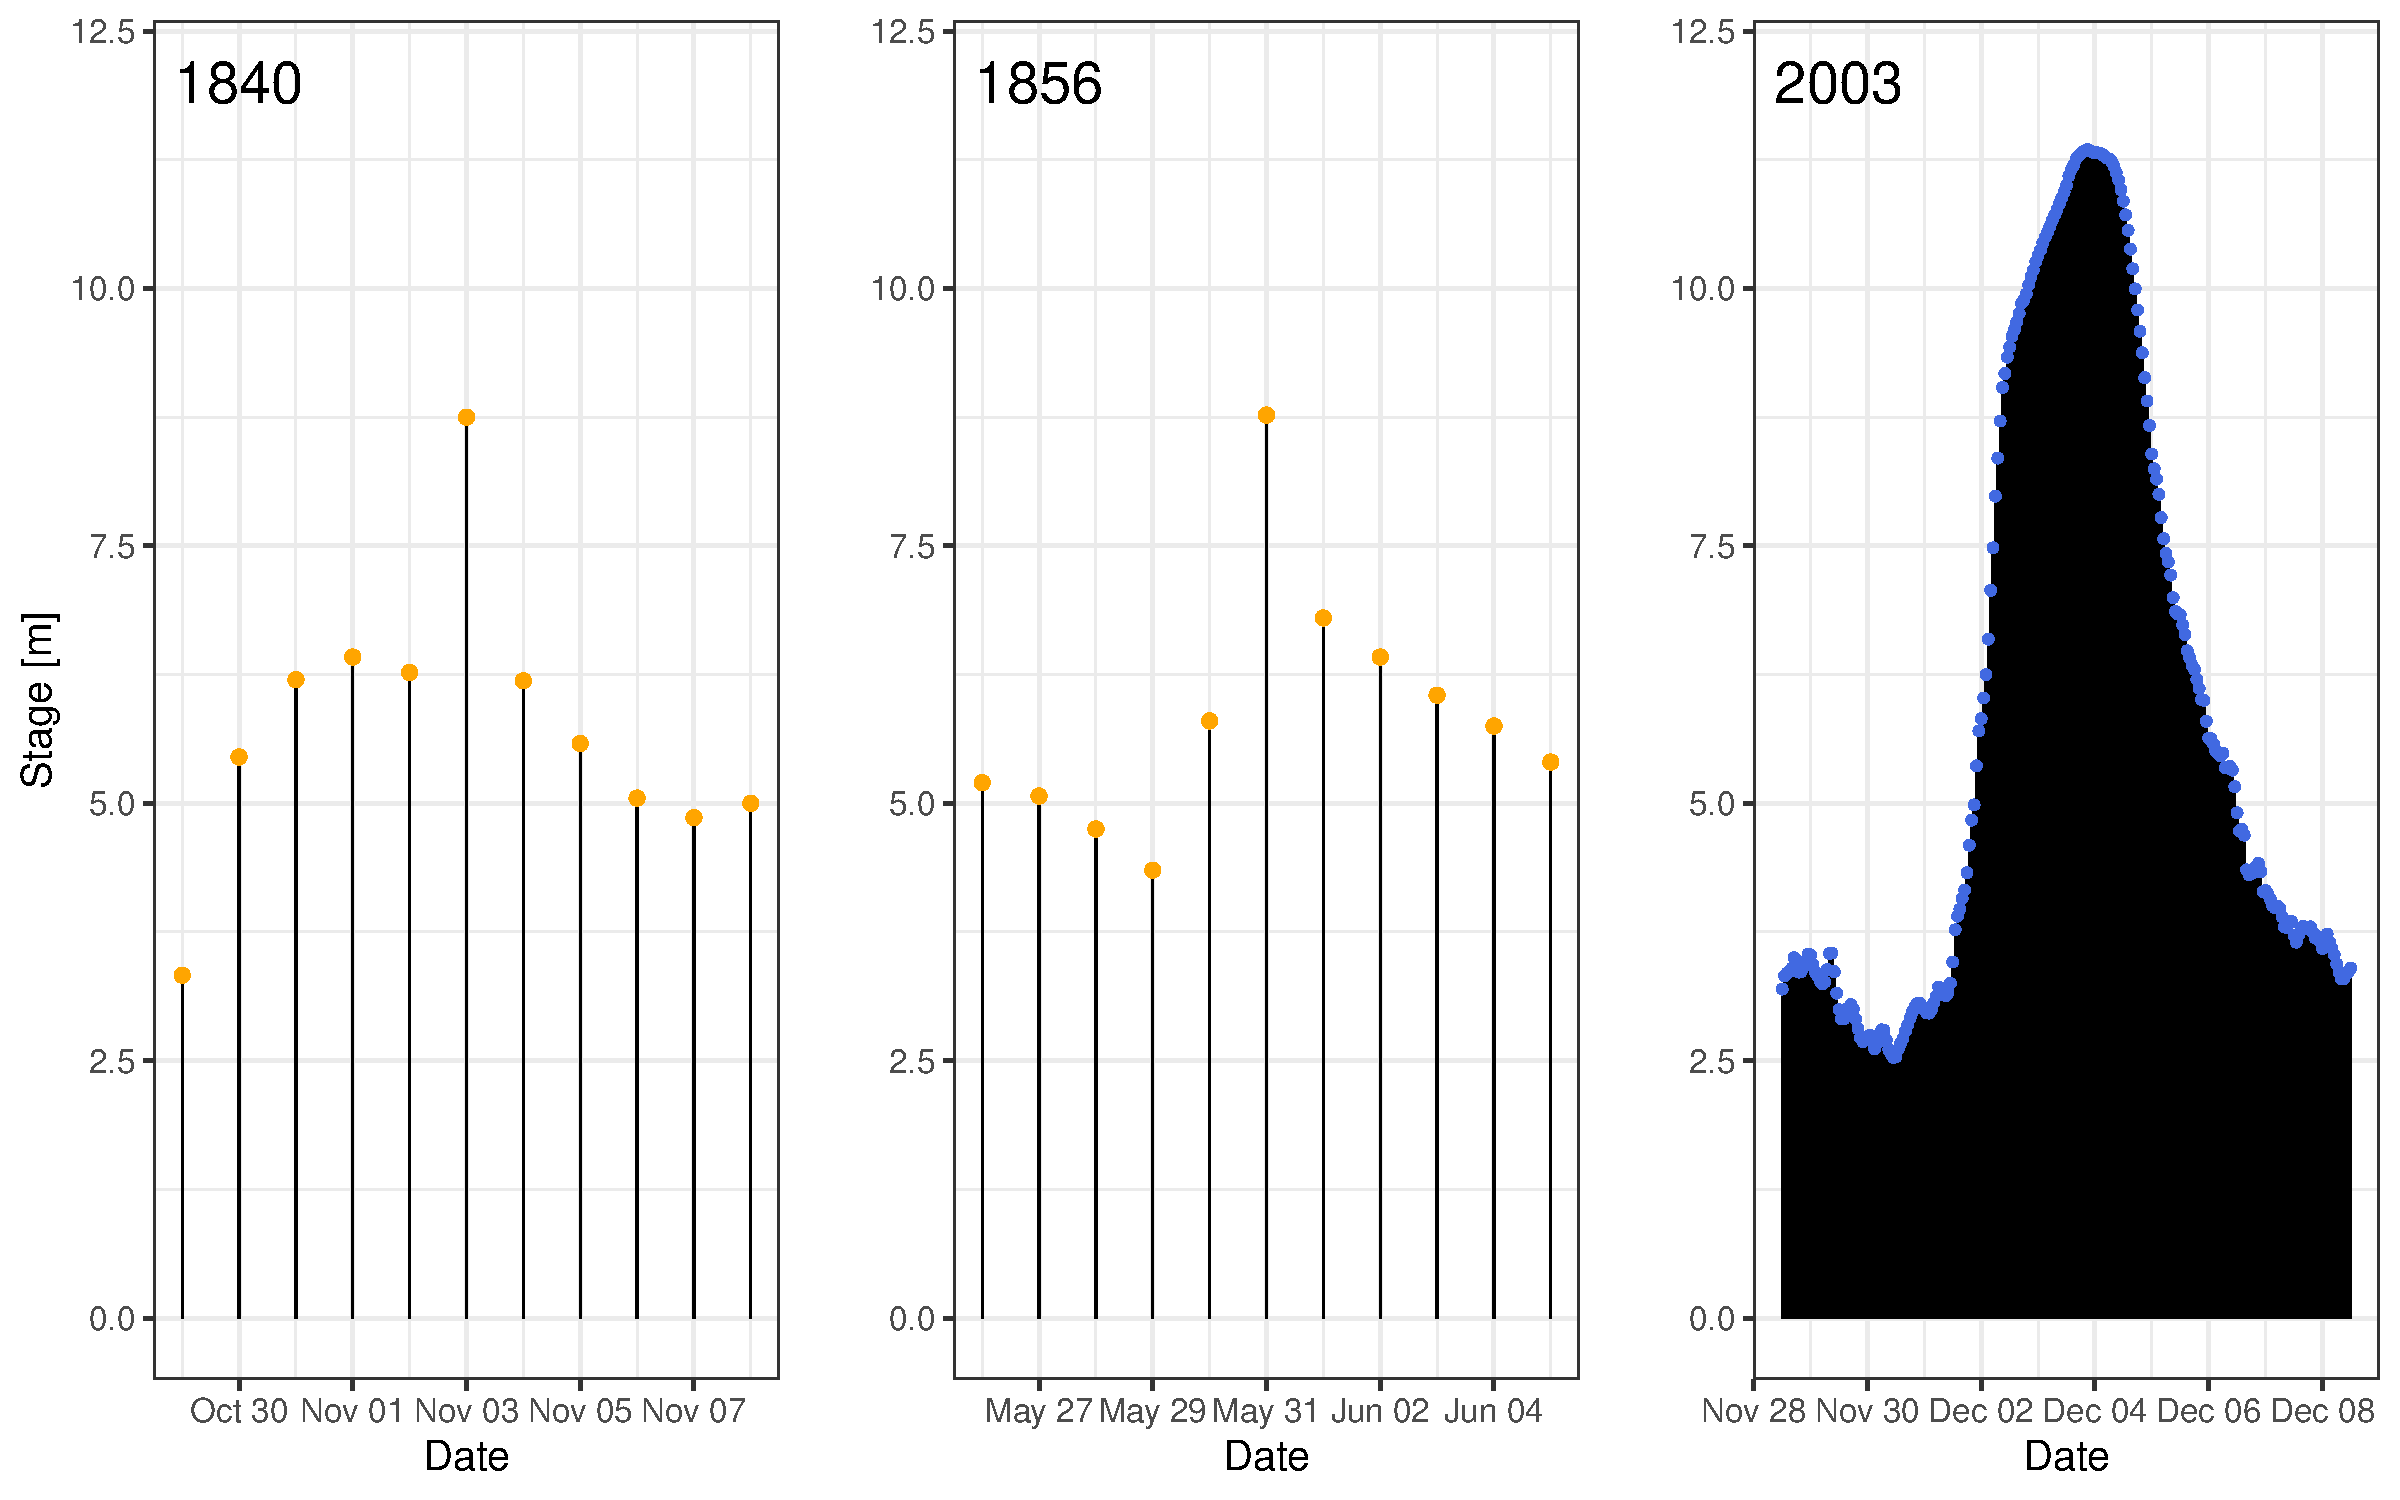
\includegraphics[width=\linewidth]{Supplementary/FloodStages.pdf}
	    \caption{Stage measurements of the 3 greatest floods recorded at Beaucaire. 1840 and 1856 floods were recorded at Pont de Beaucaire gauge, where only daily measurements are available, but the peak stage is known. 2003 flood was recorded at Beaucaire Restitution gauge for which hourly measurements are available. The datum and the cross-section geometry of the two gauges are different, which explains the differences between the stages of the XIX\textsuperscript{th} and the XXI\textsuperscript{th} centuries}
	    \label{fig:FloodStages}
	\end{figure}
		
	
	\begin{figure}
		\centering
		\begin{subfigure}{.8\textwidth}
            \centering
            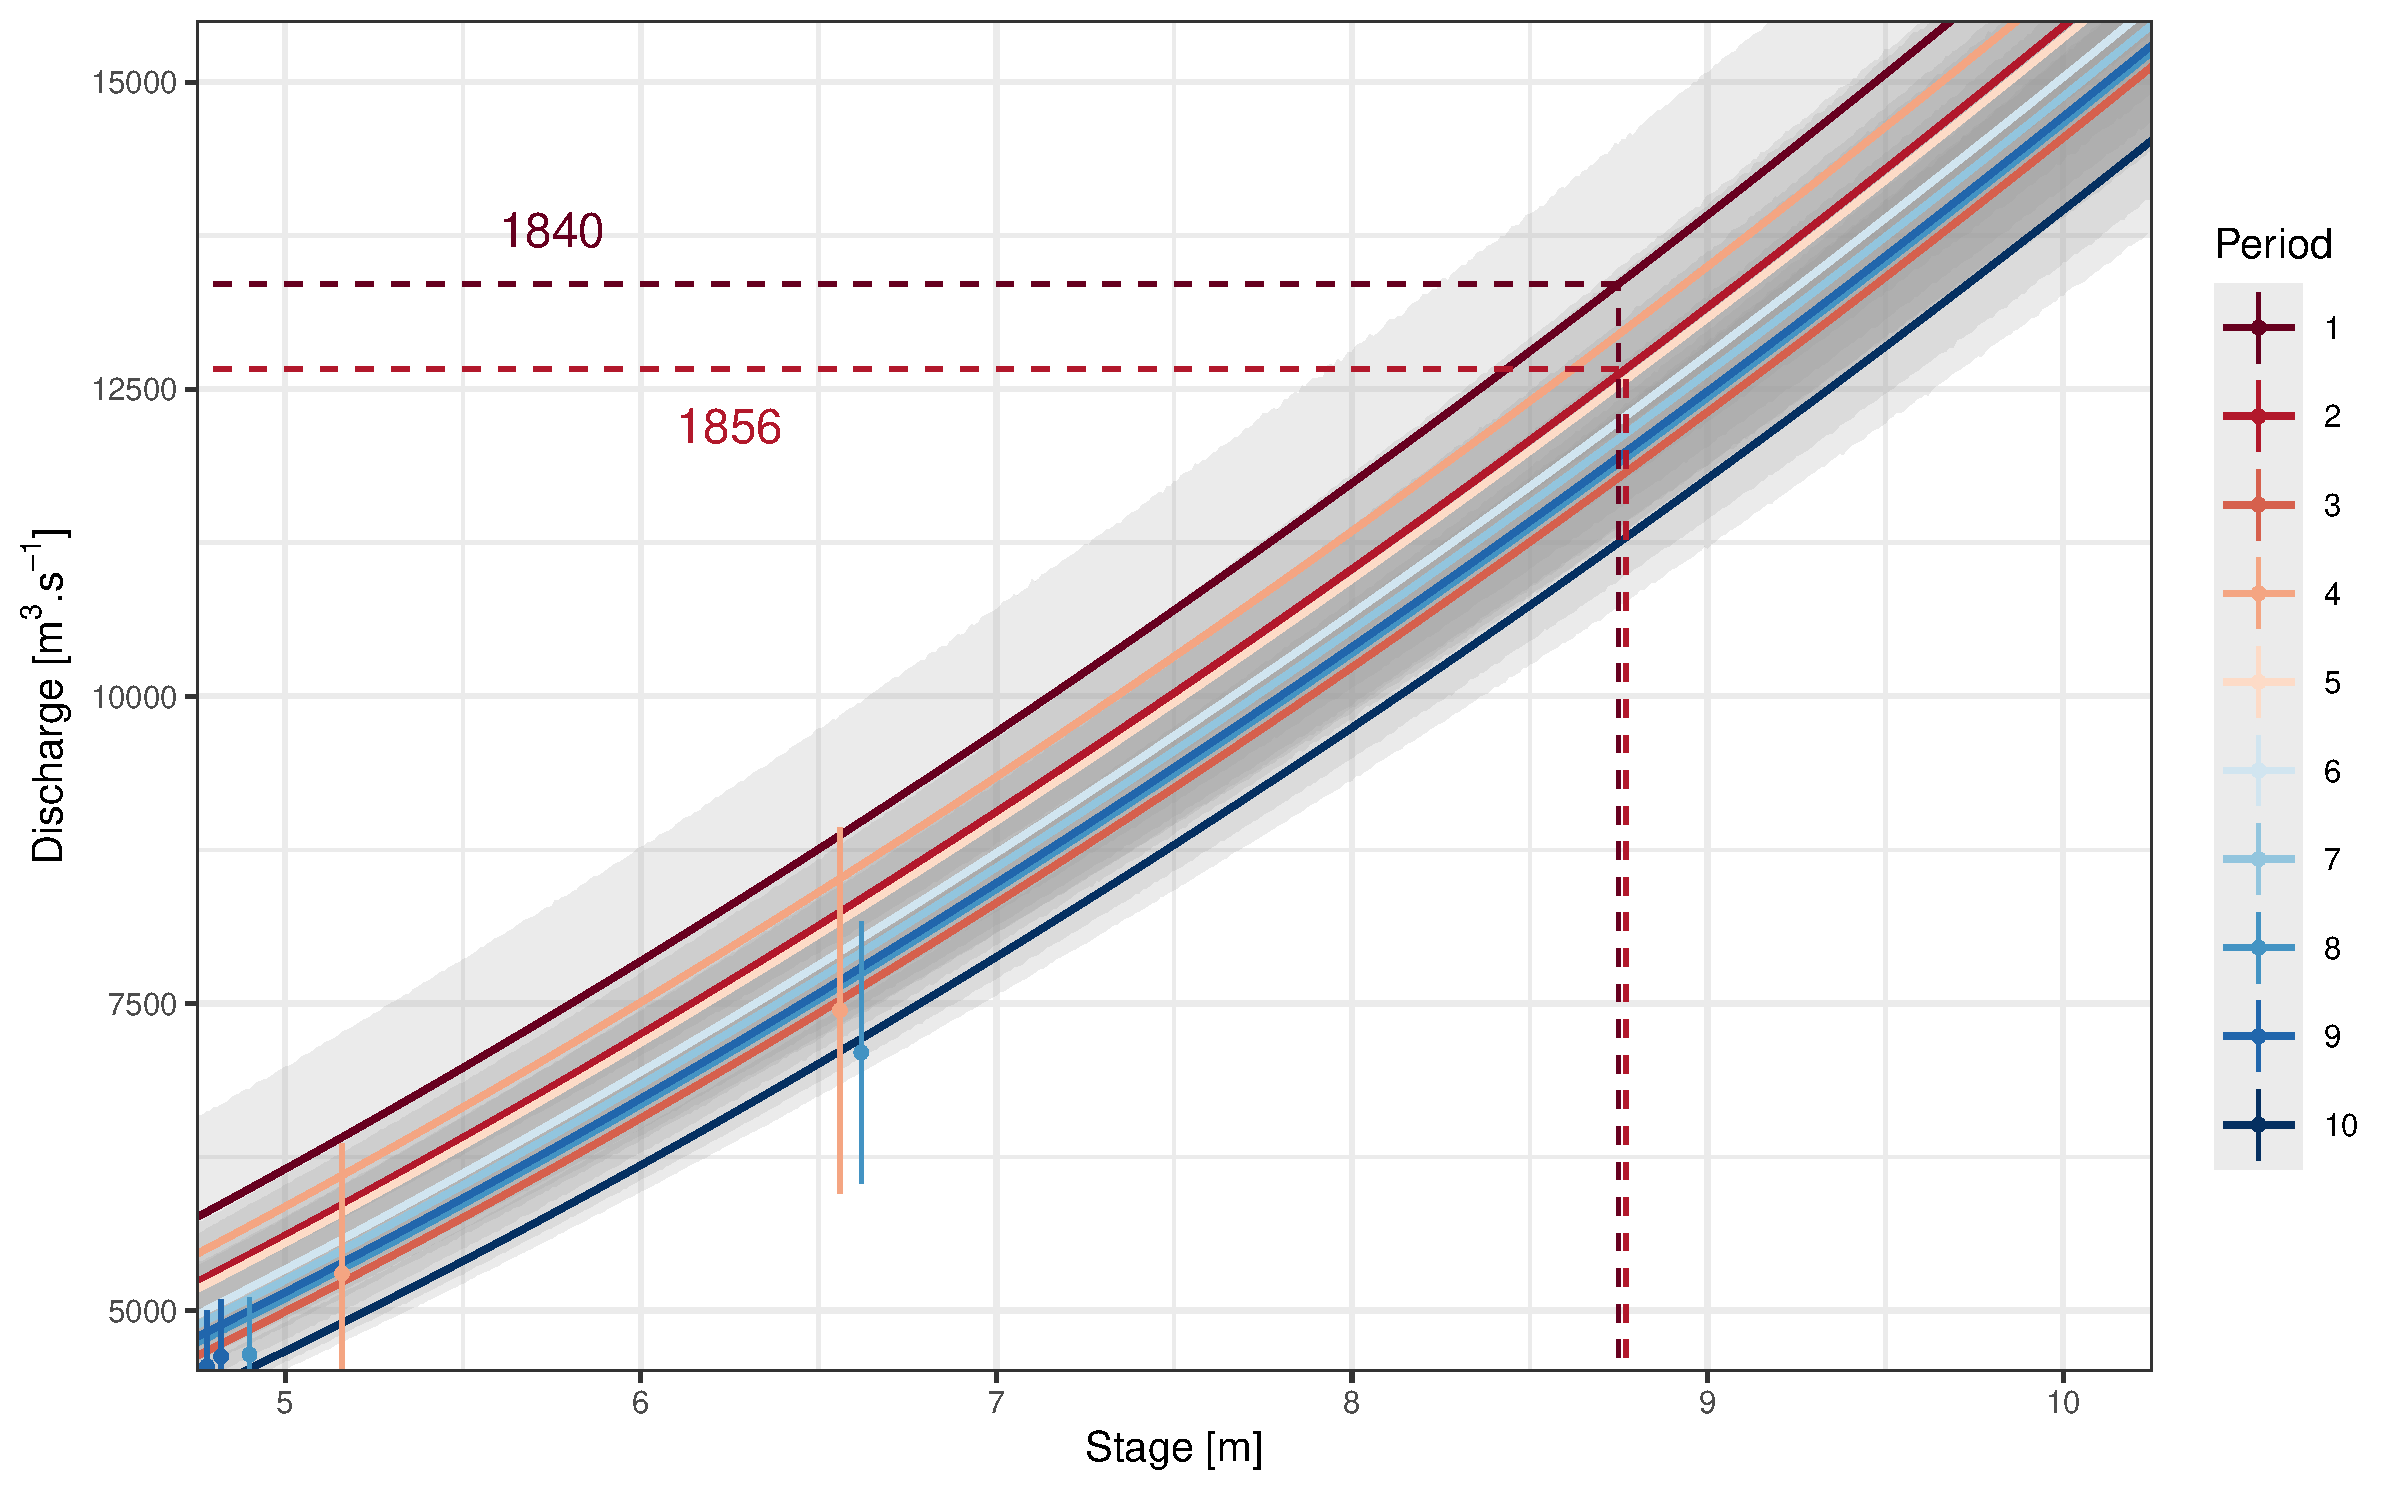
\includegraphics[width=\linewidth]{Supplementary/RC_Pt_zoom.pdf}
            \caption{}
            \label{subfig:RcPtZoom}
        \end{subfigure}
        \begin{subfigure}{0.8\textwidth}	
            \centering
            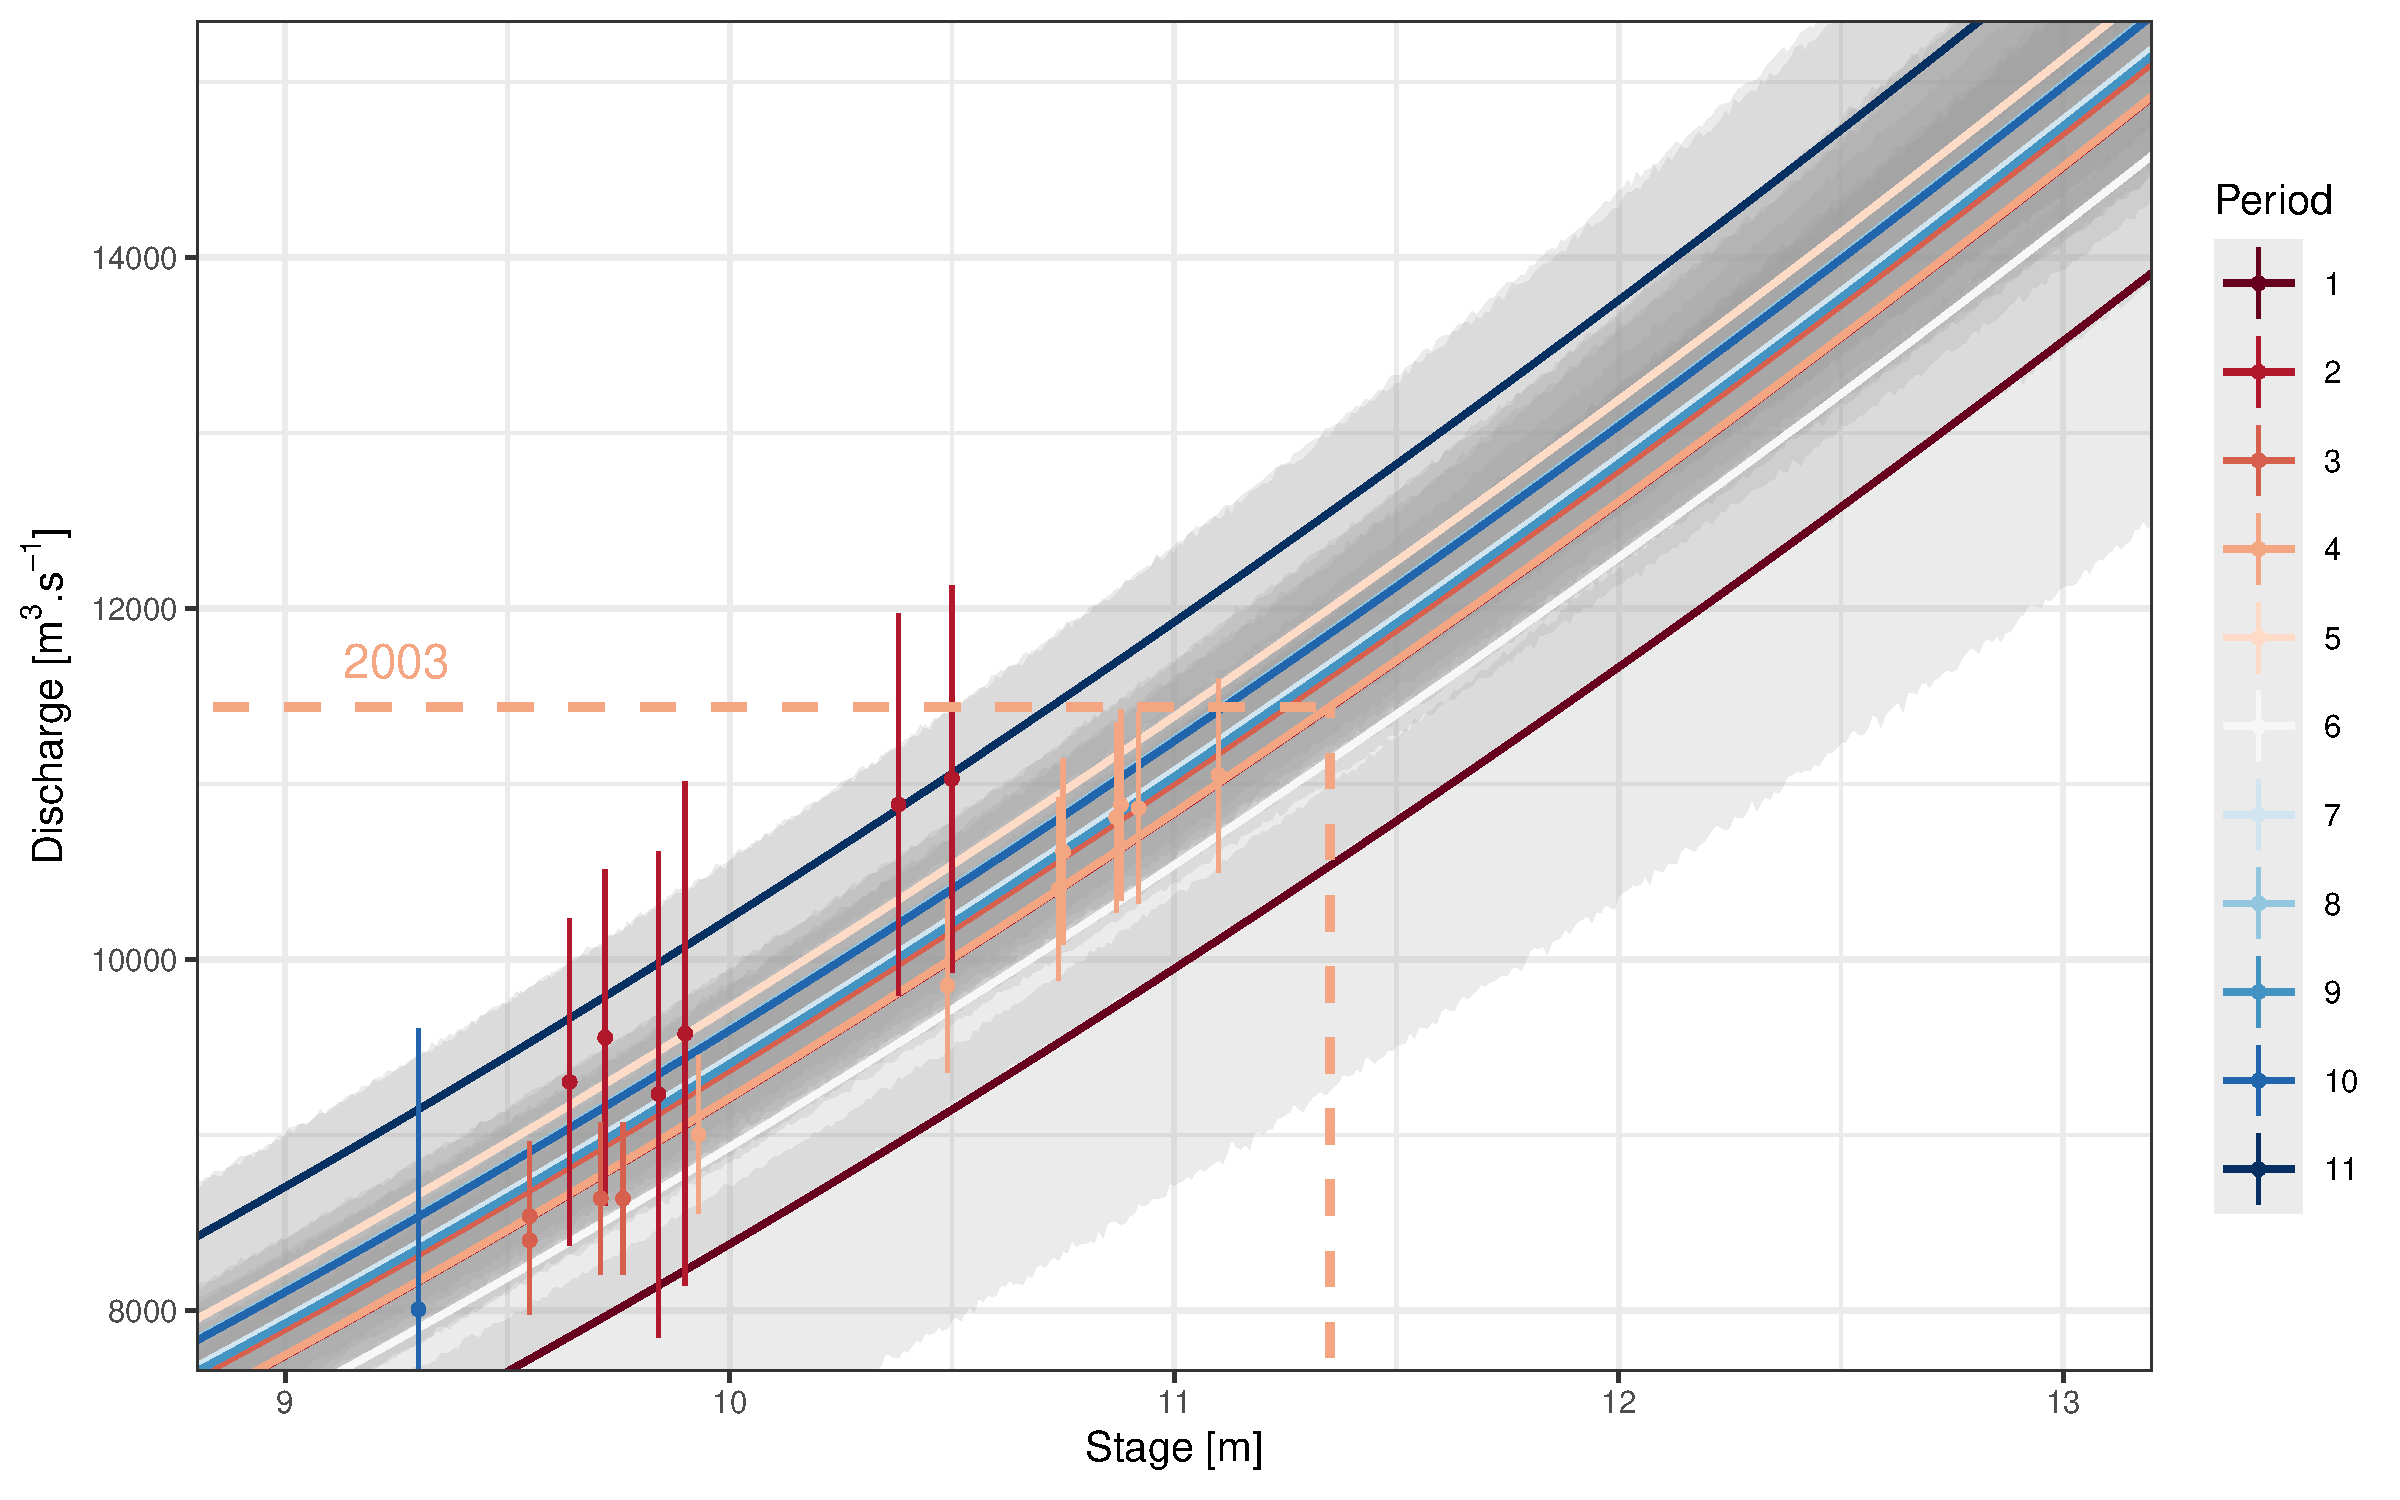
\includegraphics[width=\linewidth]{Supplementary/RC_Res_zoom.pdf}
            \caption{}
            \label{subfig:RcResZoom}
        \end{subfigure}
        \caption{Magnified rating curves of Pont de Beaucaire (a) and Beaucaire Restitution gauges (b) with 95\% uncertainty (in grey) with respect to maxpost values (solid lines). Dots with error bars represent the gaugings with 95\% uncertainty. Stable stage-discharge periods are numbered from the oldest to the latest (see table 5 in the article).}
	\end{figure}
	

	
	\begin{figure}[h]
		\centering
		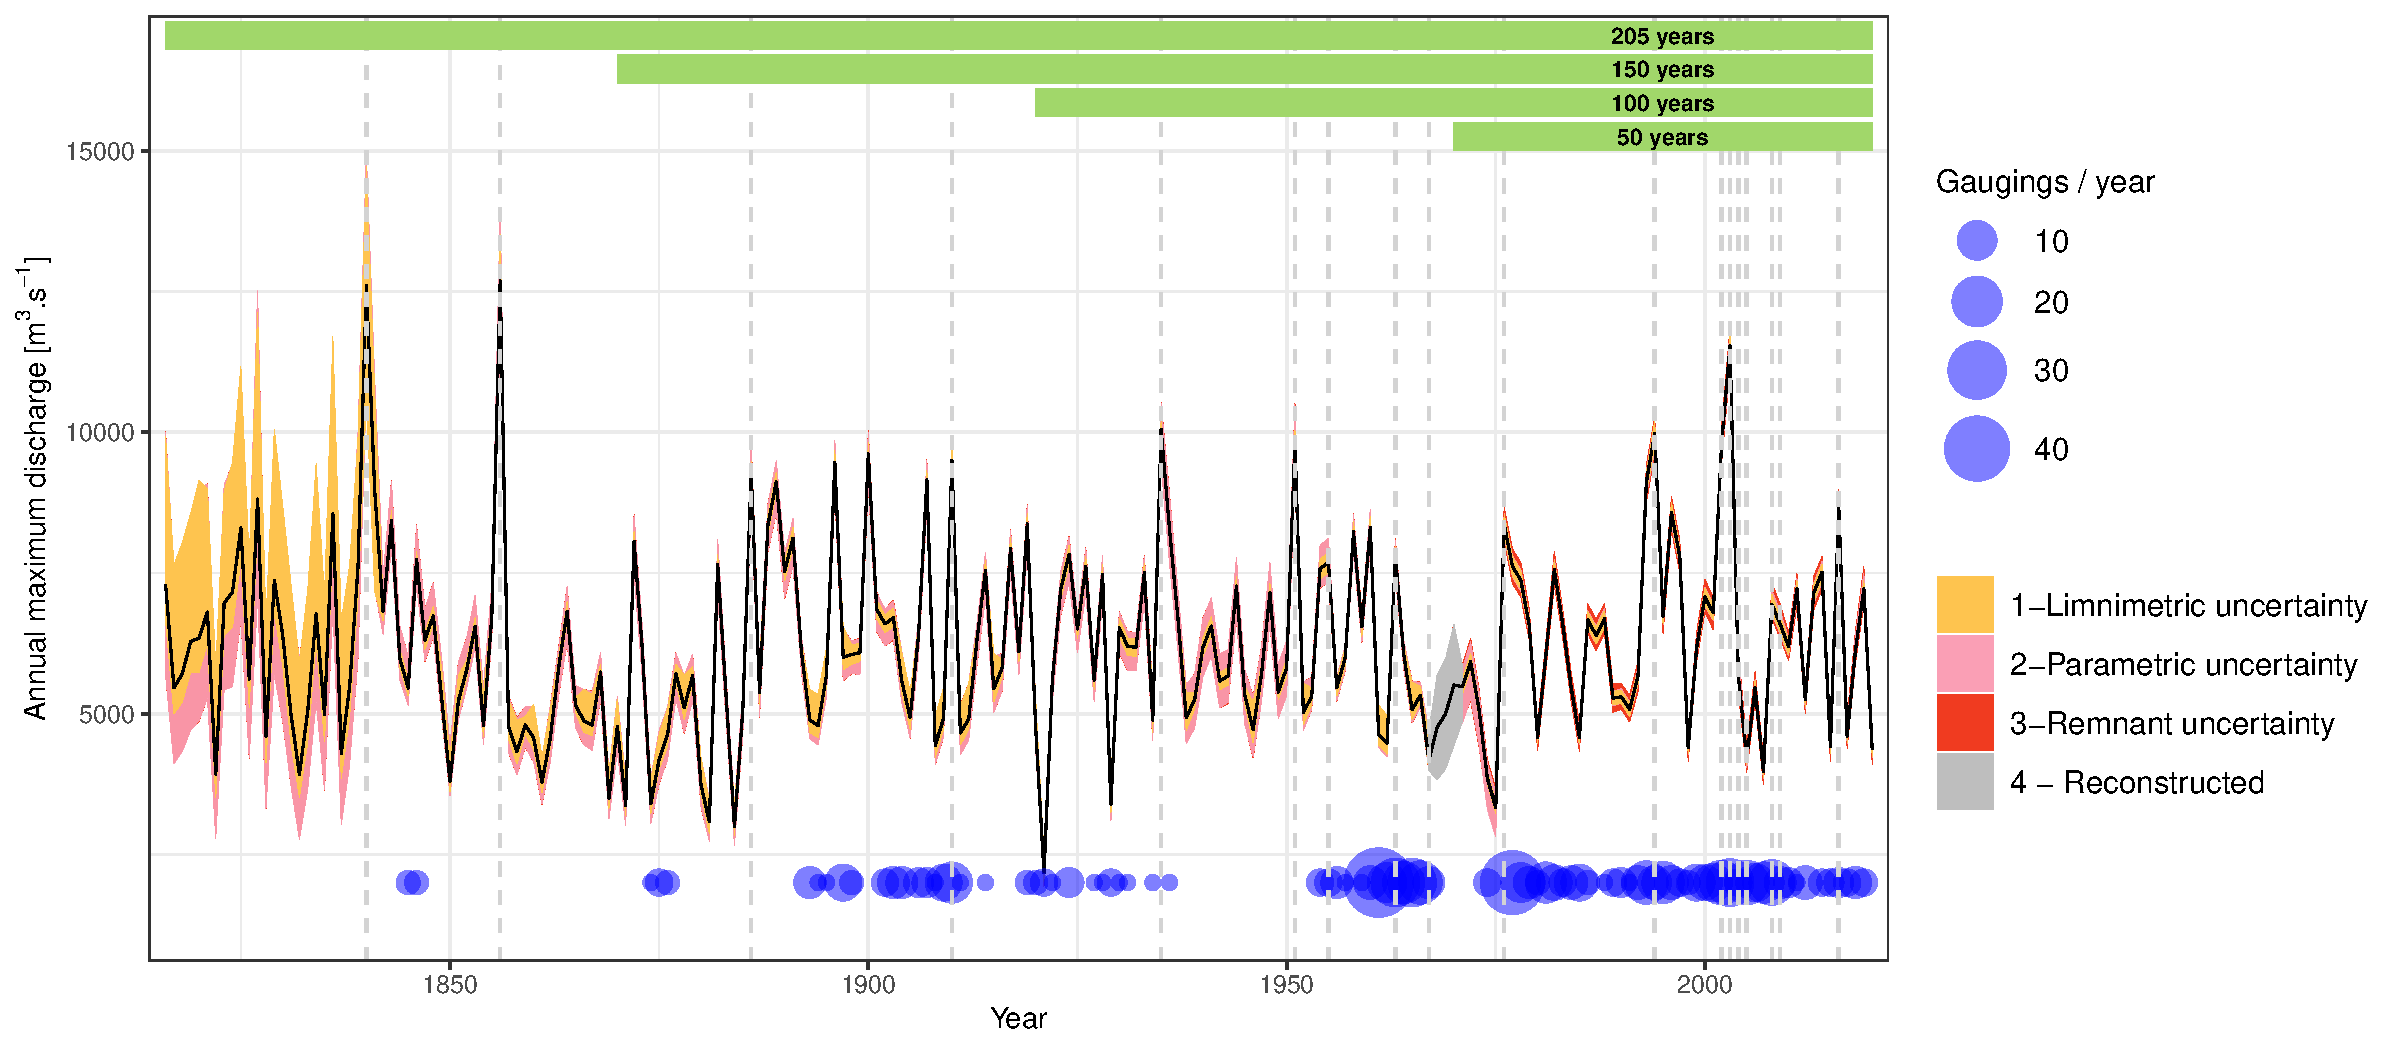
\includegraphics[width=1\linewidth]{Supplementary/IC_AMAX_Both_Bands.pdf}
	    \caption{AMAX maxpost discharges (black solid line) time series with 95\% uncertainties from three different sources at Beaucaire (1816-2020). The three greatest floods are indicated. Vertical dotted lines represent rating shifts from table 5 and green bands represent the sub-samples used in section 4.5.3.}
	    \label{fig:AMAX_Bands}
	\end{figure}
	
	
\end{document}
